\section{Implementazione hardware}

La fase di sviluppo di questo progetto ha subito molti problemi nella parte hardware, portando a vari prototipi e infine alla riduzione della complessità del progetto stesso.\\

Infatti si è passati da un sistema di sensorizzazione completa di una mano, con 2 IMU per dito più 3 IMU per modellare il movimento del palmo (in particolare il piegamento sul metacarpo dato dal pollice e quello dato dal mignolo), per un totale di 13 IMU e 2 multiplexer, a un progetto semplificato su un singolo dito, per un totale di 3 IMU e 1 multiplexer.

\subsection{Primo prototipo}

\begin{figure}[H]
    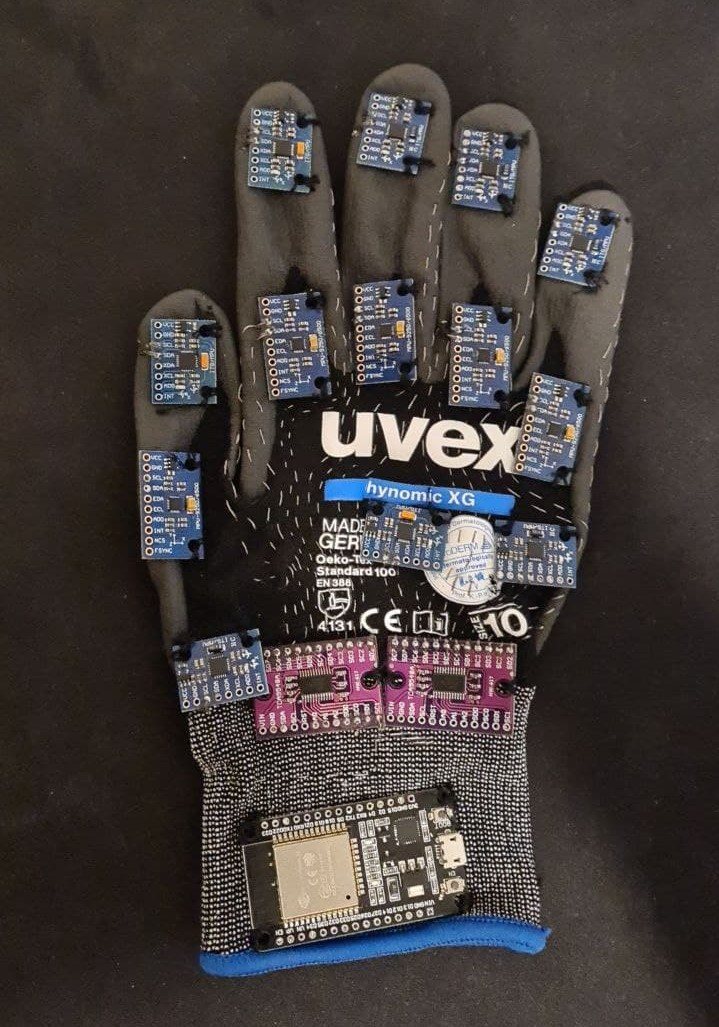
\includegraphics[scale=0.35]{immagini/prototipo1.jpg}
    \centering
    \caption{V1}
\end{figure}

Inizialmente si era pensato di utilizzare un filo conduttivo per collegare insieme i dispositivi posti sul guanto: questo avrebbe consentito di cucire più saldamente i vari componenti, utilizzando sia cuciture normali che il filo conduttivo stesso, e allo stesso tempo avrebbe dato al guanto un aspetto più \textit{tight fit}, non avendo cavi che si estendono oltre il volume del guanto.\\
Purtroppo questa strada ha portato a molti problemi di interferenze tra circuiti troppo vicini, e ancor più grave la presenza di cortocircuiti, tra cui almeno uno sui molteplici fili che collegavano i pin VCC e GND per l'alimentazione delle IMU, causando drastici cali di tensione che permettevano l'accensione di appena 2/3 IMU su 12 (sparse, non sullo stesso dito).\\

Per cercare di risolvere il problema si è ricorsi all'uso di un multimetro per l'individuazione dei cortocircuiti, e una melassa isolante da spalmare sui fili. Siccome anche questo non ha portato ai risultati sperati, si è deciso di ritentare modificando il progetto.

\begin{figure}[H]
    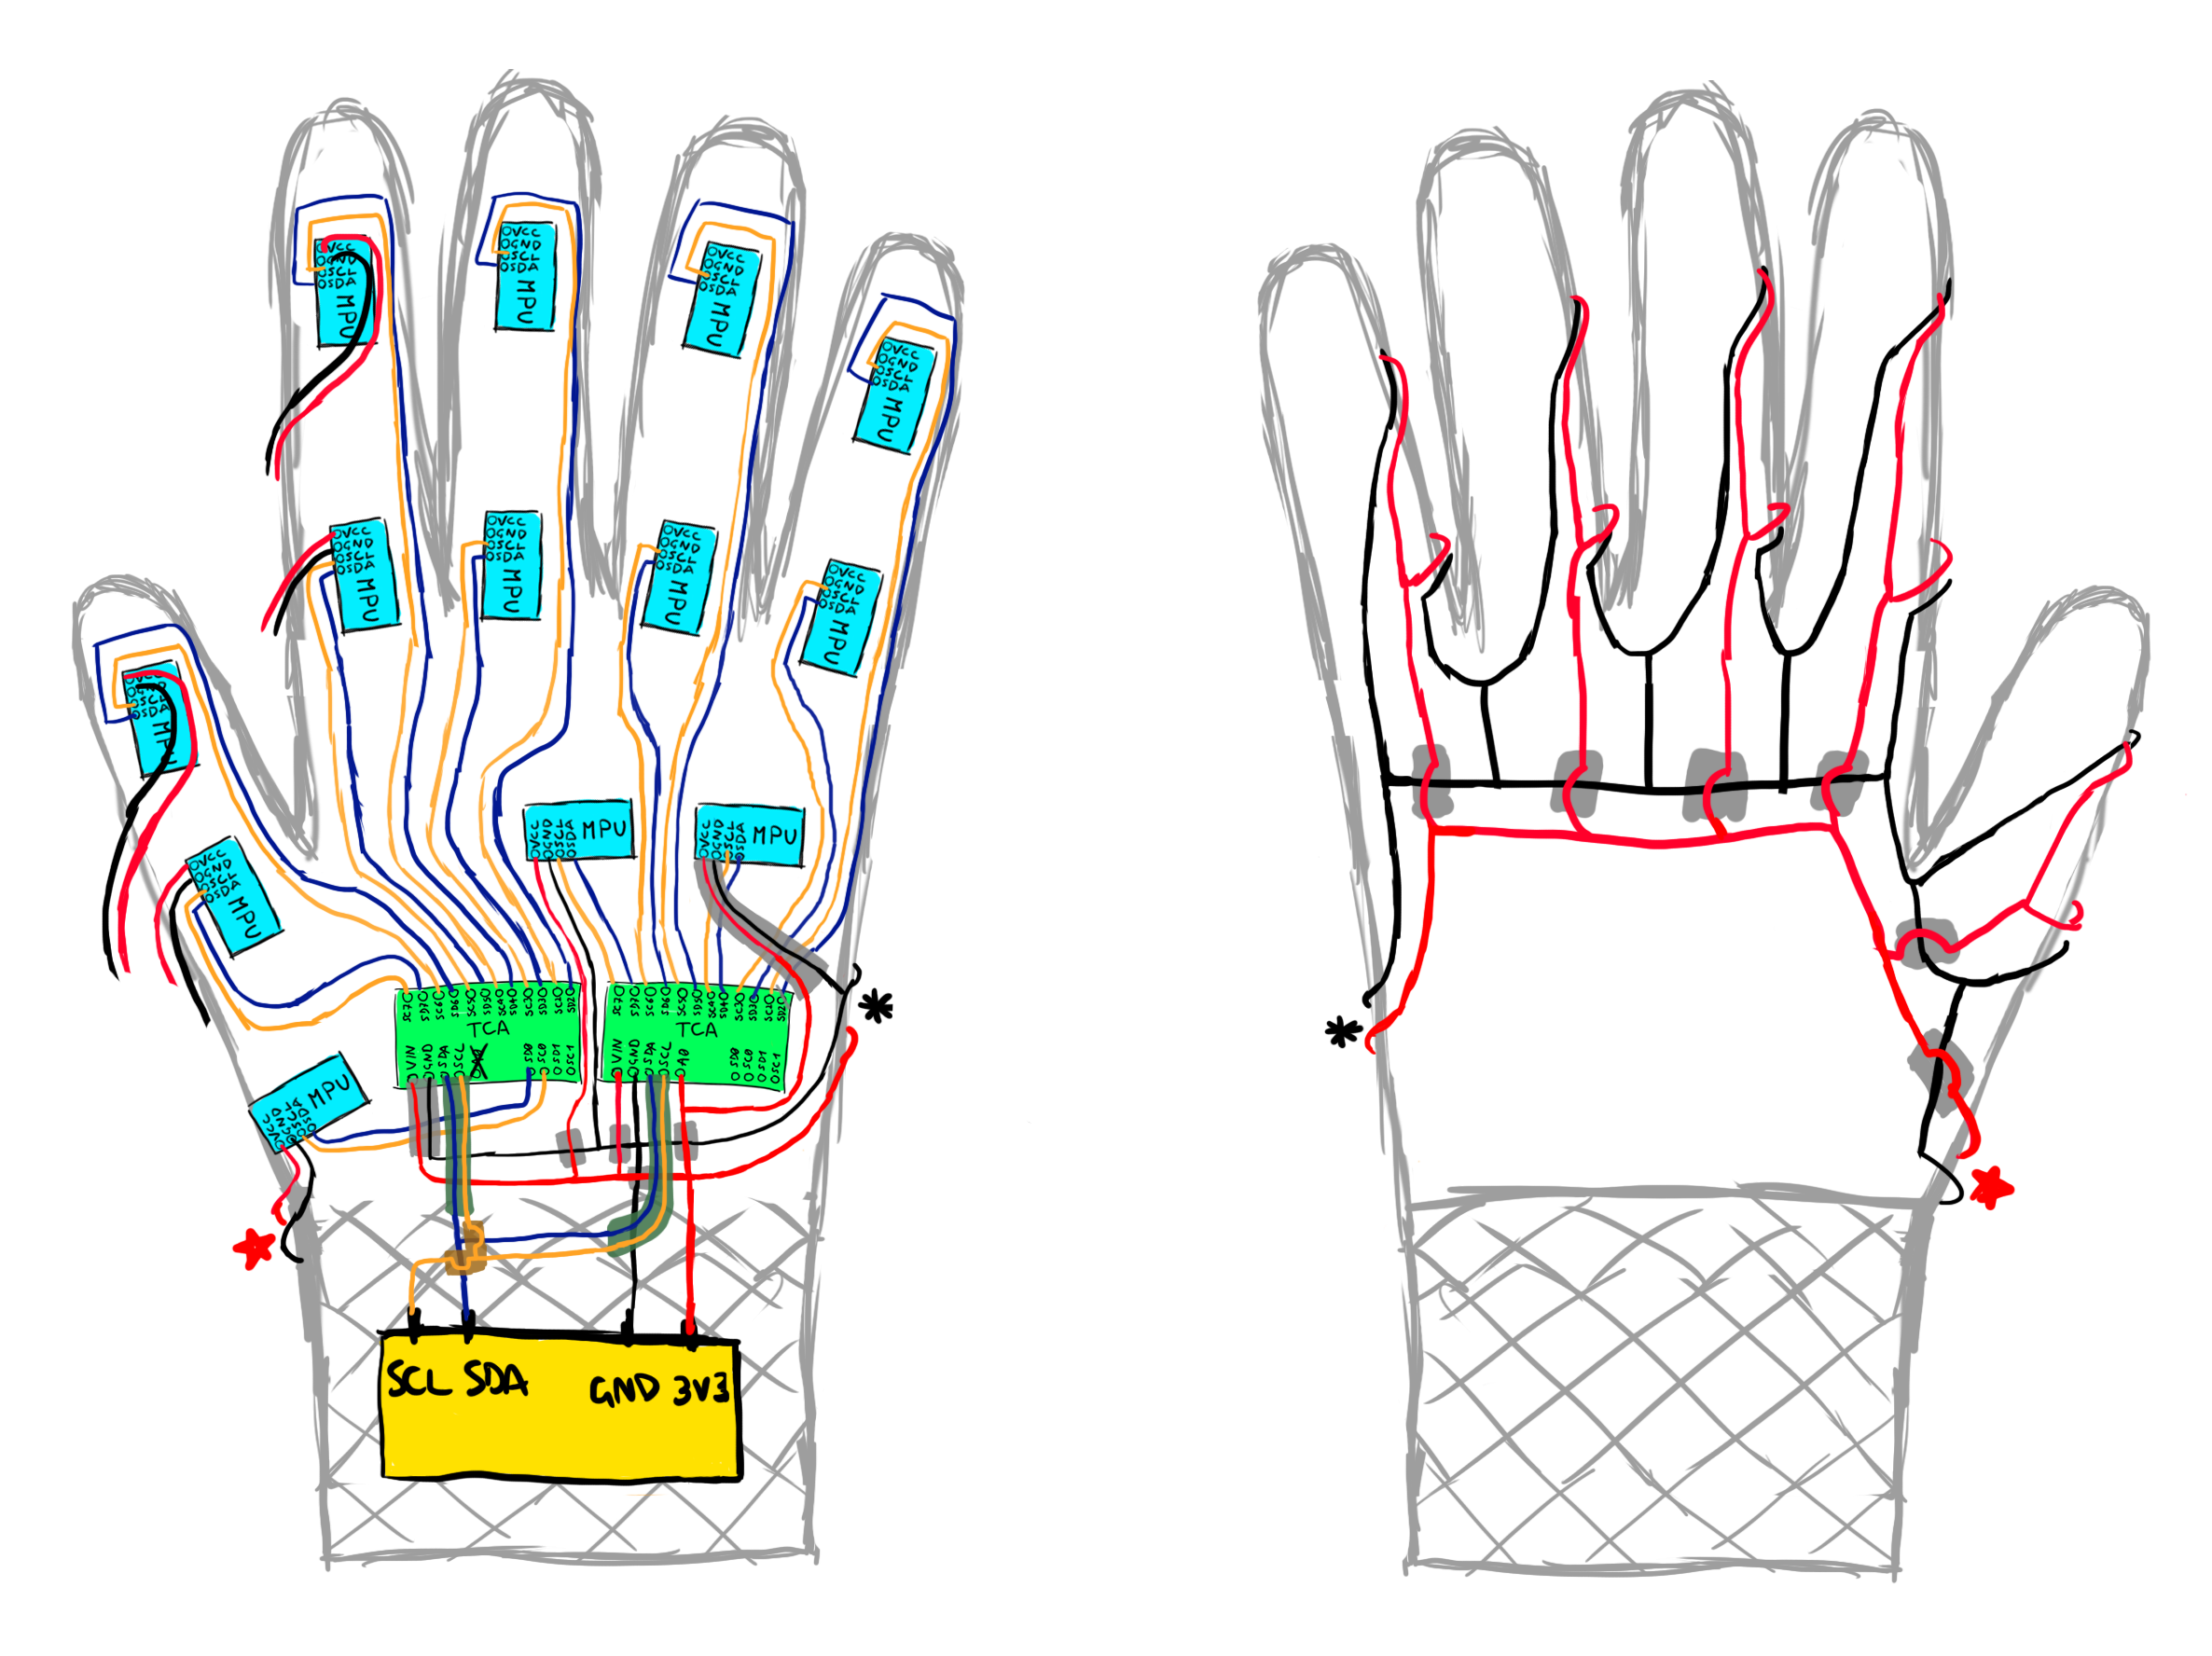
\includegraphics[scale=0.35]{immagini/guanto_schema.png}
    \centering
    \caption{V1 - schema dei collegamenti}
\end{figure}

\clearpage

\subsection{Secondo prototipo}

\begin{figure}[H]
    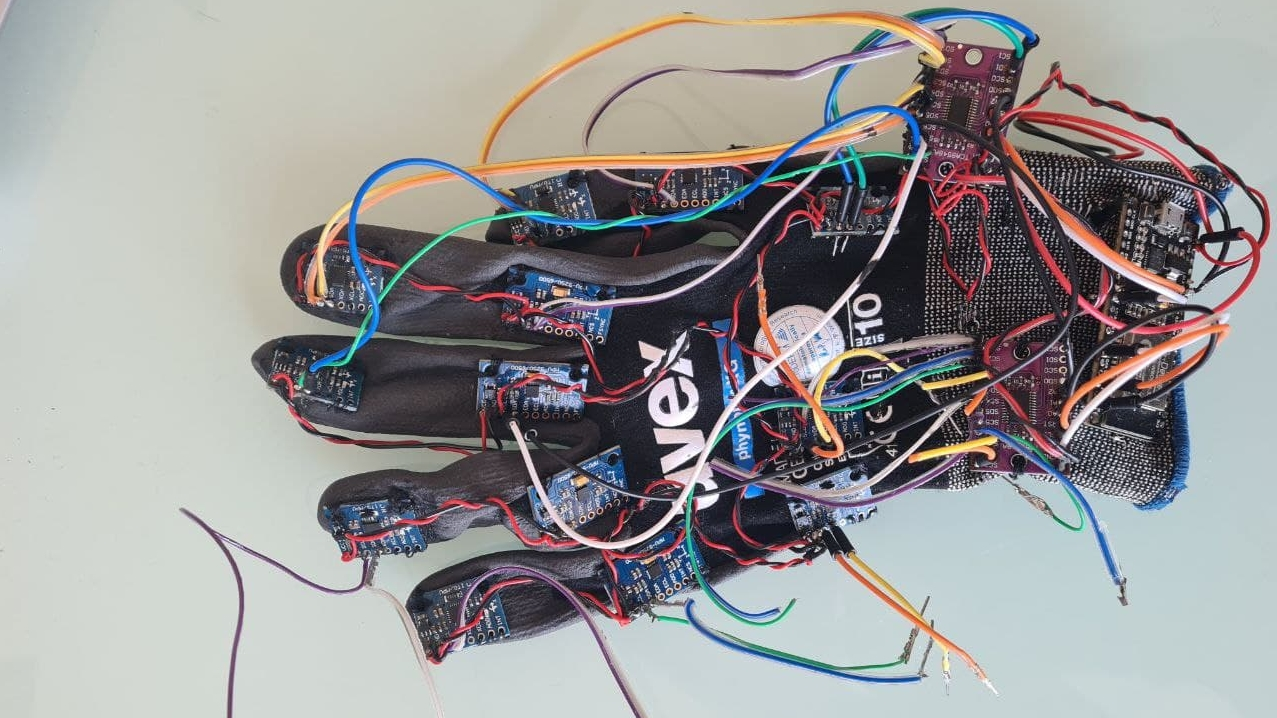
\includegraphics[scale=0.35]{immagini/prototipo2.jpg}
    \centering
    \caption{V2}
\end{figure}

Per il secondo prototipo del guanto si è abbandonata l'idea del filo per cucire conduttivo, sostituendolo con dei normali cavetti isolati, e in tal modo si è riusciti ad arrivare in una configurazione tale per cui tutte le IMU si accendessero senza problemi.\\

Ci sono stati tuttavia altri problemi imprevisti: alcuni collegamenti I2C perdevano sporadicamente segnale anche per minimi movimenti del guanto, e il programma di recezione dati riceveva zeri su tutte le misure dell'IMU; i cavi inoltre sono stati saldati e crimpati per avere collegamenti stabili ed evitare ulteriori errori, ma per effettuare operazioni di debugging è stato necessario tagliarli e ricollegarli più volte; infine, molte IMU usate avevano problemi di inizializzazione e su alcuni sensori restituivano il valore di fondoscala invece che la misura effettiva, facendo pensare dopo vari tentativi di debugging falliti che fosse l'IMU stessa ad essere non funzionante.\\

Per questi motivi si è passati a una terza versione del guanto, e poiché la probabilità di incorrere in problemi hardware aumenta proporzionalmente rispetto al numero di dispositivi utilizzati, si è quindi ritenuto necessario diminuire la complessità del progetto.

\clearpage

\subsection{Versione finale}

\begin{figure}[H]
    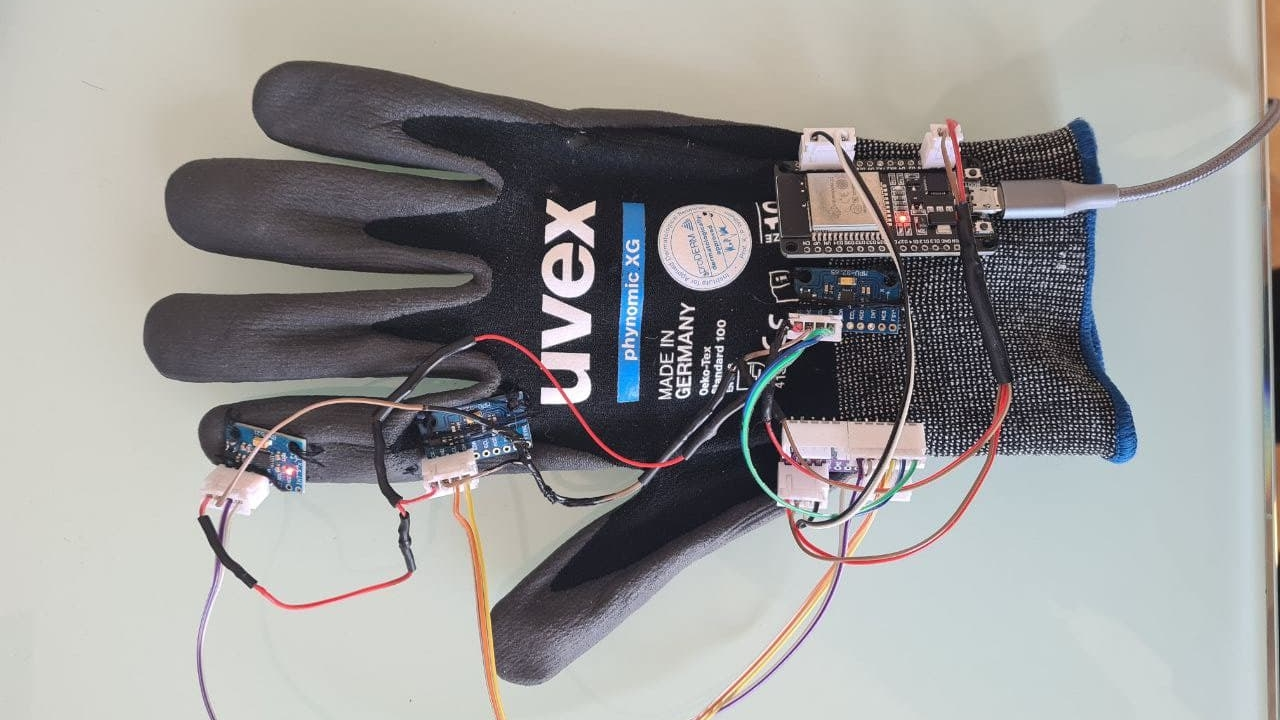
\includegraphics[scale=0.35]{immagini/prototipo3.jpg}
    \centering
    \caption{V3 - semplificato}
\end{figure}

La versione finale è quindi focalizzata su un solo dito, l'indice, e di conseguenza impiega molti meno dispositivi.\\

Tutti i dispositivi utilizzati sono stati testati in modo approfondito prima ancora di essere installati sul guanto, per assicurarsi che funzionasse correttamente.\\

Con questa versione non ci sono stati problemi, e ogni nuova IMU collegata è stata testata prima di connettere la successiva. I cavi invece di venire saldati direttamente sono stati collegati con degli header (JTS).
L'inserzione degli header JTS garantisce un collegamento solido, evitando problemi di connessioni instabili (molto presenti nel caso di I2C), ma allo stesso tempo consente di poterli scollegare e ricollegare in qualsiasi momento.\\

\clearpage